\begin{figure*}[ht]
\centering

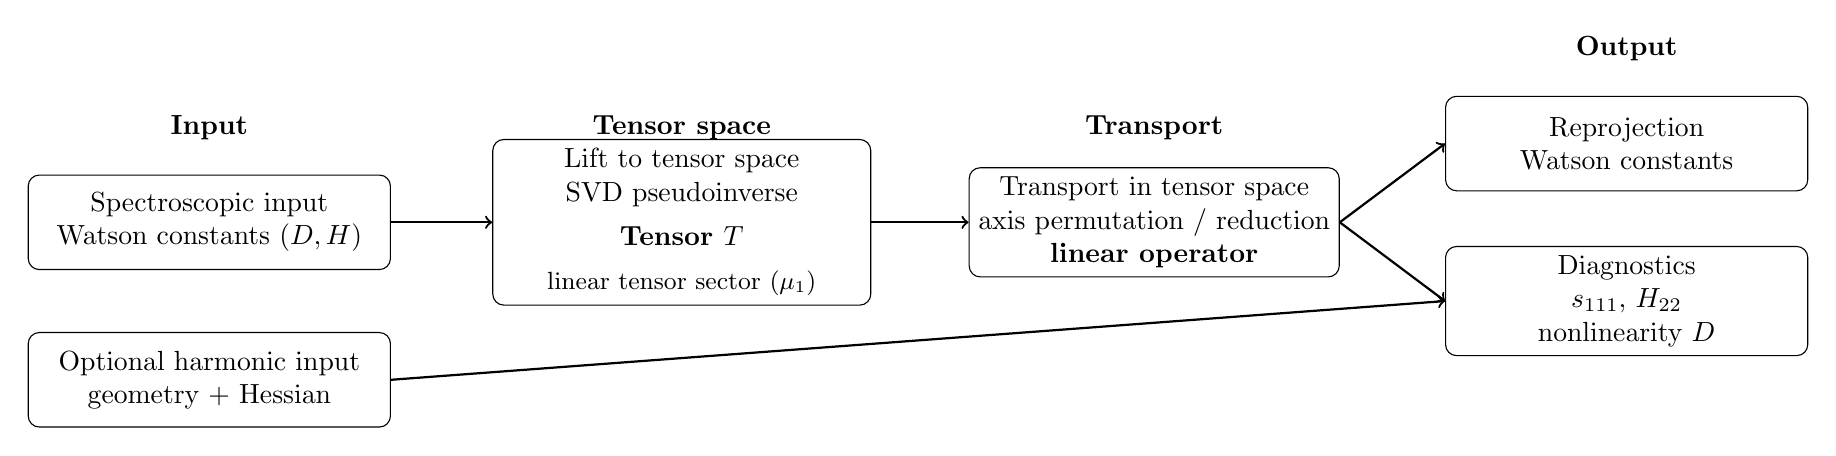
\begin{tikzpicture}[
box/.style={
rectangle,draw,rounded corners,
align=center,
minimum width=4.6cm,
minimum height=1.2cm
},
core/.style={
rectangle,draw,rounded corners,
align=center,
minimum width=4.8cm,
minimum height=1.4cm
},
arrow/.style={->, thick}
]

% =======================
% LEFT COLUMN (INPUT)
% =======================

\node[box] (fit) at (0,0)
{Spectroscopic input\\Watson constants $(D,H)$};

\node[box] (harm) at (0,-2)
{Optional harmonic input\\geometry + Hessian};

\node[draw=none] at (0,1.2) {\textbf{Input}};

% =======================
% CENTER (TENSOR)
% =======================

\node[core] (tensor) at (6,0)
{Lift to tensor space\\
SVD pseudoinverse\\[4pt]
\textbf{Tensor $T$}\\[4pt]
{\small linear tensor sector ($\mu_1$)}};

\node[draw=none] at (6,1.2) {\textbf{Tensor space}};

% =======================
% TRANSPORT
% =======================

\node[box] (transport) at (12,0)
{Transport in tensor space\\
axis permutation / reduction\\
\textbf{linear operator}};

\node[draw=none] at (12,1.2) {\textbf{Transport}};

% =======================
% OUTPUT
% =======================

\node[box] (reproj) at (18,1)
{Reprojection\\Watson constants};

\node[box] (diag) at (18,-1)
{Diagnostics\\$s_{111}$, $H_{22}$\\nonlinearity $D$};

\node[draw=none] at (18,2.2) {\textbf{Output}};

% =======================
% ARROWS
% =======================

\draw[arrow] (fit.east) -- (tensor.west);
\draw[arrow] (tensor.east) -- (transport.west);
\draw[arrow] (transport.east) -- (reproj.west);
\draw[arrow] (transport.east) -- (diag.west);
\draw[arrow] (harm.east) -- (diag.west);

\end{tikzpicture}

\caption{
Operational structure of the tensor framework. Spectroscopic parameters are lifted to a representation-independent tensor space via SVD-based pseudoinverse reconstruction, defining tensor representatives within the linear sector generated by $\mu_1$. Representation changes are performed as linear operations in tensor space, and the results are reprojected onto the desired Watson parametrization. Optional harmonic input enables the evaluation of diagnostic quantities that probe the breakdown of the linear tensor regime.
}

\label{fig:workflow}
\end{figure*}

